\chapter{ادراک شنیداری، مقیاس مل و ضرایب \eng{MFCC}}

تا اینجا سیگنال گفتار را از دید فیزیکی بررسی کردیم (شکل موج، فوریه، هارمونیک، فرمنت، فضای واکه‌ای) و طیفی دیدیم که همهٔ فرکانس‌ها را یکسان می‌دید. در این جلسه ویژگی‌های \term{سیستم شنوایی انسان}{Human Auditory System} را وارد استخراج ویژگی می‌کنیم. حاصل کار مقیاس مل، بانک فیلتر مل، لگاریتم و در نهایت \term{ضرایب کپسترال فرکانس مل}{Mel-Frequency Cepstral Coefficients} یا \eng{MFCC} است که در جلسات بعد هم بارها به آن برمی‌گردیم.

\begin{exambox}{نقشهٔ راه جلسه}
(۱) چرا شنوایی را مدل کنیم؟ (۲) نقشهٔ تونوتوپیک حلزون؛ (۳) مقیاس مل و بانک فیلتر مثلثی؛ (۴) لگاریتم برای ادراک غیرخطی بلندی؛ (۵) افزونگی ویژگی‌ها، \eng{DCT} و پیدایش \eng{MFCC}؛ (۶) کپستروم؛ (۷) کاربردها و رابطهٔ \eng{MFCC} با یادگیری ماشین.
\end{exambox}

%====================================================================
\section{چرا باید ادراک شنیداری انسان را در نظر بگیریم؟}
%====================================================================

تبدیل فوریه می‌گوید هر مؤلفهٔ فرکانسی چه سهمی دارد، بی‌آنکه بپرسد انسان کدام فرکانس‌ها را بهتر تشخیص می‌دهد. انسان جوان و سالم صداهایی را در حدود \textbf{۲۰ هرتز تا ۲۰ کیلوهرتز} می‌شنود، و باید دو چیز را از هم جدا کرد:
\begin{itemize}
  \item \textbf{وجود فیزیکی ارتعاش}: پدیده‌ای که طبق قوانین فیزیک رخ می‌دهد؛
  \item \textbf{ادراک شنیداری ارتعاش}: فرایندی که ارتعاش را از دستگاه شنوایی عبور می‌دهد و در مغز به تجربهٔ شنیدن تبدیل می‌کند.
\end{itemize}
مثال کلاس از بینایی: چراغی که با فرکانس بسیار زیاد چشمک می‌زند را پیوسته روشن می‌بینیم، هرچند از نظر فیزیکی همچنان خاموش و روشن می‌شود.

%====================================================================
\section{نقشهٔ تونوتوپیک حلزون گوش}
%====================================================================

صدا از گوش خارجی و میانی می‌گذرد و در \term{حلزون گوش}{Cochlea} موجی روی \term{غشای پایه}{Basilar Membrane} پدید می‌آورد. نقاط مختلف این غشا به فرکانس‌های مختلف حساس‌اند؛ به این سازمان‌دهی \term{نقشهٔ تونوتوپیک}{Tonotopic Map} می‌گویند.

\begin{figure}[htbp]
  \centering
  \fbox{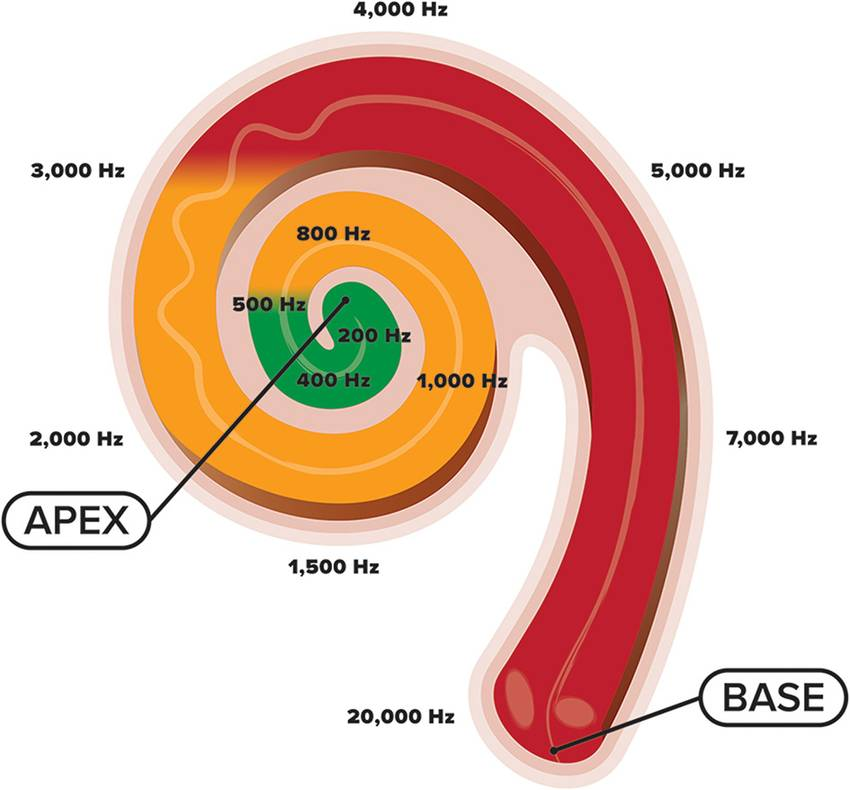
\includegraphics[width=0.46\textwidth]{../assets/figures/ch05-cochlea-tonotopic.png}}\hspace{0.03\textwidth}
  \fbox{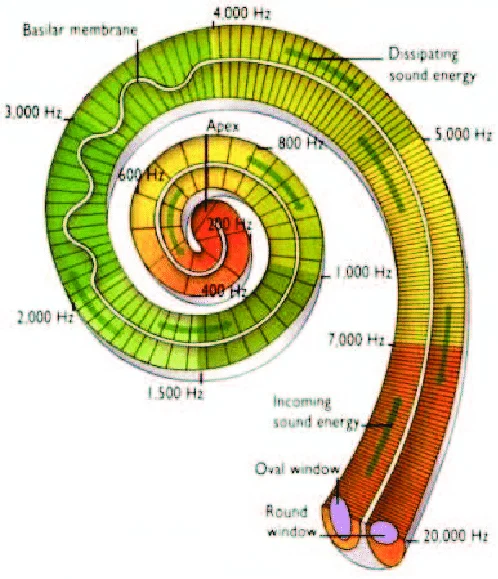
\includegraphics[width=0.38\textwidth]{../assets/figures/ch05-basilar-membrane.png}}
  \caption{نقشهٔ تونوتوپیک حلزون گوش. رأس (\eng{Apex}) مربوط به فرکانس‌های بم و قاعده (\eng{Base}) نزدیک دریچه‌های بیضی و گرد مربوط به فرکانس‌های زیر است. \textit{(برگرفته از تختهٔ کلاس)}}
  \label{fig:cochlea}
\end{figure}

\begin{correctionbox}{دقت در خواندن شکل}
عدد نزدیک رأس (حدود ۲۰۰ هرتز) حد پایین واقعی شنوایی نیست؛ شنوایی تا حدود ۲۰ هرتز ادامه دارد. همچنین فاصلهٔ مکانی روی غشای پایه تقریباً با \emph{لگاریتم فرکانس} متناسب است (نه خطی)؛ همین ریشهٔ فیزیولوژیک مقیاس مل است.
\end{correctionbox}

\subsection{تفکیک نابرابر فرکانس‌های بم و زیر}
ادراک تغییرات فرکانسی خطی نیست. دو تغییر $100\to200$ هرتز و $5100\to5200$ هرتز هر دو ۱۰۰ هرتز اختلاف دارند، اما اولی برای گوش چشمگیر و دومی تقریباً نامحسوس است؛ یعنی تفاوت ادراکی به \emph{محدودهٔ فرکانسی} هم بستگی دارد، نه فقط به اختلاف عددی. مثال‌های کلاس: تغییر کوچک در صدای موتور (فرکانس پایین) به‌سادگی شنیده می‌شود، ولی تغییر کوچک فرکانس یک سوت (فرکانس بالا) دشوارتر. گوش در فرکانس‌های پایین (زیر حدود ۱۰۰۰ هرتز) بسیار دقیق است و در فرکانس‌های بالا (بالای حدود ۴۰۰۰ هرتز) کمتر.

\begin{correctionbox}{دقت علمی}
در فرکانس‌های بالا تفکیک گوش تقریباً نسبت‌محور است. تغییر ۱۰۰ هرتز در ۵ کیلوهرتز برای شنوندهٔ آموزش‌دیده هنوز قابل‌تشخیص است؛ درست‌تر این است که از نظر ادراکی \emph{بسیار کوچک‌تر} از تغییر ۱۰۰ به ۲۰۰ هرتز به‌نظر می‌رسد. مقیاس مل همین را مدل می‌کند.
\end{correctionbox}

\textbf{پیامد:} در فرکانس‌های پایین بازه‌های باریک و در بالا بازه‌های پهن‌تر می‌خواهیم؛ این مبنای مقیاس مل است.

%====================================================================
\section{مرور سه ویژگی \eng{Pitch}، \eng{Formant} و \eng{Intensity} در \eng{Praat}}
%====================================================================

استاد روی یک سیگنال در \eng{Praat} (فرمنت‌ها: نقطه‌های قرمز؛ \eng{pitch}: خط آبی؛ شدت: خط زرد) سه ویژگی را مرور کرد:
\begin{itemize}
  \item \term{فرمنت}{Formant}: نواحی تشدید طیفی ($F_1$، $F_2$، $F_3$) که برای ساخت فضای واکه‌ای به کار رفتند.
  \item \term{پیچ}{Pitch}: ادراک زیر و بمی؛ با فرکانس پایه $F_0$ (کمیت فیزیکی، تناوب سیگنال) مرتبط است ولی با آن یکی نیست.
  \item \term{شدت}{Intensity}: معیار قدرت کلی صوت در هر لحظه (فریاد: شدت زیاد، صحبت آرام: شدت کم).
\end{itemize}

\begin{table}[htbp]
\centering
\caption{کمیت‌های فیزیکی و ادراکی که باید از هم جدا نگه داشته شوند.}
\begin{tabular}{p{4cm}p{4.5cm}p{4cm}}
\toprule
\textbf{کمیت فیزیکی} & \textbf{کمیت ادراکی} & \textbf{توضیح} \\
\midrule
فرکانس پایه \eng{($F_0$)} & زیر و بمی (\eng{Pitch}) & تناوب موج در برابر احساس زیر/بم \\
شدت (\eng{Intensity}) & بلندی (\eng{Loudness}) & توان فیزیکی در برابر بلندی احساس‌شده \\
فرمنت‌ها / شکل طیف & رنگ صدا (\eng{Timbre}) & تشدیدهای مجرای صوتی \\
\bottomrule
\end{tabular}
\end{table}

زیر و بمی با بلندی یکی نیست: می‌توان با صدای زیر ولی آرام، یا بم و پرشدت صحبت کرد.

\begin{exambox}{پرسش و پاسخ: چرا خط \eng{pitch} گاهی بالاتر از نقطه‌های فرمنت است؟}
چون این نمودارها با \emph{محورهای مختلف} (یک مقیاس برای \eng{pitch}، یکی برای فرمنت) روی یک تصویر رسم می‌شوند؛ بالاتر بودن خط روی صفحه دلیل بزرگ‌تر بودن مقدار فرکانسی نیست. نحوهٔ محاسبهٔ کانتور این ویژگی‌ها جلسهٔ بعد بررسی می‌شود.
\end{exambox}

%====================================================================
\section{کم‌شنوایی فرکانس‌های بالا با افزایش سن}
%====================================================================

چون قاعدهٔ حلزون به فرکانس‌های بالا مربوط است، آسیب به آن شنیدن صداهای زیر را کم می‌کند؛ کم‌شنوایی فرکانس‌های بالا در سنین بالا رایج است و \term{پیرگوشی}{Presbycusis} نام دارد. توضیح کلاس: سلول‌های ناحیهٔ قاعده در «خط مقدم» ضربه‌های مکانیکی‌اند و زودتر تحلیل می‌روند.

\begin{correctionbox}{دقت علمی}
الگوی کلی درست است، اما علت آن چندعاملی است (از دست رفتن سلول‌های مویی، تحلیل رگ‌ها، نورون‌های عصب شنوایی، نویز، ژنتیک و غیره)؛ توضیح کلاس را «سازوکارهای محتمل» بدانید نه علت قطعی. نمونهٔ عملی: همخوان‌های بی‌واک مانند \eng{/s/} و \eng{/f/} انرژی‌شان در فرکانس‌های بالاست و برای افراد دچار پیرگوشی سخت‌تر تفکیک می‌شوند.
\end{correctionbox}

%====================================================================
\section{مقیاس مل}
%====================================================================

\begin{definitionbox}{مقیاس مل}
\term{مقیاس مل}{Mel Scale} یک \textbf{نگاشت غیرخطی} از فرکانس فیزیکی (هرتز) به مقیاس ادراکی (مل) است که فرکانس‌های بالا را «فشرده» می‌کند تا فاصله‌های برابر روی محور مل تقریباً با تفاوت‌های ادراکی برابر در زیر و بمی متناظر باشند. نام آن از \eng{melody} گرفته شده است.
\end{definitionbox}

\begin{correctionbox}{فرمول مقیاس مل}
مقیاس مل را استیونز، فولکمن و نیومن (۱۹۳۷) از آزمایش‌های قضاوت زیر و بمی معرفی کردند. رایج‌ترین تقریب تحلیلی (که در کلاس به‌صورت عددی بیان نشد):
\[
m = 2595\,\log_{10}\!\Big(1+\frac{f}{700}\Big)
\qquad\Longleftrightarrow\qquad
f = 700\big(10^{\,m/2595}-1\big).
\]
۱۰۰۰ هرتز به ۱۰۰۰ مل نگاشت می‌شود. قراردادهای دیگری هم وجود دارد (مثلاً نسخهٔ اسلینی)، پس خروجی کتابخانه‌ها ممکن است اندکی فرق کند.
\end{correctionbox}

تابع در فرکانس‌های پایین (زیر حدود ۱ کیلوهرتز) تقریباً خطی و در فرکانس‌های بالاتر لگاریتمی است.

\begin{figure}[htbp]
  \centering
  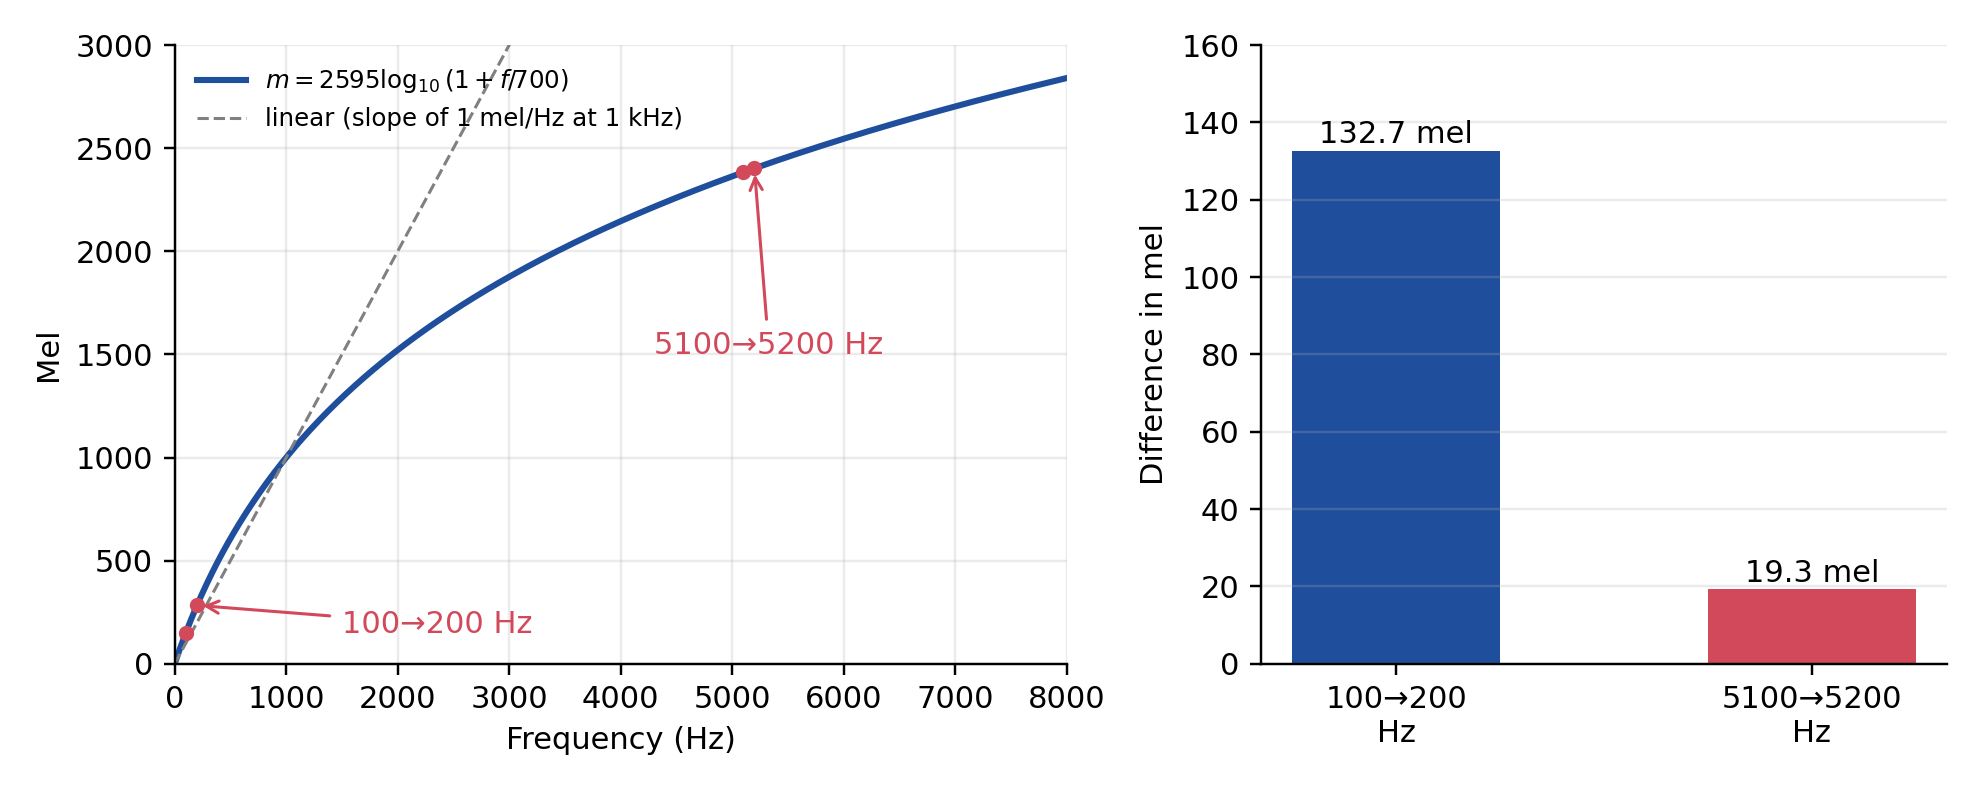
\includegraphics[width=0.95\textwidth]{../assets/figures/ch05-mel-vs-hz.png}
  \caption{چپ: منحنی تبدیل هرتز به مل. راست: همان دو تغییر ۱۰۰ هرتزی در مقیاس مل ($132.7$ مل در برابر $19.3$ مل). (شکل افزوده)}
  \label{fig:melcurve}
\end{figure}

\begin{addedbox}{مثال عددی: تبدیل هرتز به مل}
\begin{center}
\begin{tabular}{rrrrrrr}
\toprule
$f$ (هرتز) & 100 & 200 & 1000 & 2000 & 5100 & 8000 \\
\midrule
$m$ (مل) & $150.5$ & $283.2$ & $1000.0$ & $1521.4$ & $2383.1$ & $2840.0$ \\
\bottomrule
\end{tabular}
\end{center}
بازهٔ ۰ تا ۸ کیلوهرتز فقط به حدود ۲۸۴۰ مل نگاشت می‌شود و نیمی از آن (۰ تا ۱۴۲۰ مل) زیر حدود ۱۷۶۰ هرتز است؛ یعنی مل به فرکانس‌های پایین «فضای بیشتری» می‌دهد.
\end{addedbox}

%====================================================================
\section{بانک فیلتر مل}
%====================================================================

\term{بانک فیلتر مل}{Mel Filterbank} مجموعه‌ای از فیلترهای مثلثی هم‌پوشان روی محور فرکانس است. هر فیلتر یک بازهٔ فرکانسی را پوشش می‌دهد و از آن \emph{یک عدد} (انرژی آن باند) می‌سازد.

\subsection{وزن‌دهی مثلثی}
وزن هر فیلتر در ابتدای بازه نزدیک صفر، در مرکز بیشینه (معمولاً ۱) و در انتها دوباره صفر است؛ پس فرکانس‌های نزدیک مرکز سهم بیشتری دارند. مقدار طیفی هر فرکانس در وزن متناظر ضرب و حاصل‌ها جمع می‌شوند:
\[
S_m=\sum_{k} H_m[k]\,P[k],
\]
که $P[k]$ طیف توان و $H_m[k]$ وزن فیلتر $m$ام است.

\begin{exambox}{مثال عددی کلاس: خروجی یک فیلتر}
فیلتری سه مؤلفهٔ طیفی با مقدارهای ۴، ۸ و ۶ و وزن‌های $0.5$، ۱ و $0.5$ دریافت می‌کند (اعداد آموزشی‌اند):
\[
M_1=(4\times0.5)+(8\times1)+(6\times0.5)=2+8+3=13 .
\]
به‌جای سه مقدار، یک عدد داریم؛ این کار برای همهٔ فیلترهای بانک تکرار می‌شود.
\end{exambox}

\subsection{چرا فیلترها هم‌پوشان‌اند؟}
تا اطلاعات فرکانس‌های نزدیک مرز دو باند ناگهان حذف یا دچار پرش نشود. مثال تخته: اگر مرز دو باند ۳۰۰ هرتز و فیلترها مستطیلی بدون هم‌پوشانی باشند، تغییر ۱ هرتزی (۲۹۹ به ۳۰۱) مؤلفه را ناگهان از یک فیلتر به فیلتر دیگر می‌برد و خروجی‌ها می‌پرند؛ با مثلث‌های هم‌پوشان فقط تغییری هموار و کوچک رخ می‌دهد.

\subsection{چرا عرض فیلترها یکسان نیست؟}
مهم‌ترین نکتهٔ بانک فیلتر مل: روی محور \emph{خطی} فرکانس، فیلترها در فرکانس‌های پایین باریک و در فرکانس‌های بالا پهن‌اند (دقت در فرکانس‌های بالا کمتر است). دلیل: فیلترها روی \emph{محور مل} یکسان و هم‌فاصله‌اند و با بازگشت به هرتز در بالا پهن می‌شوند. این همان ایدهٔ نقشهٔ تونوتوپیک است.

\begin{figure}[htbp]
  \centering
  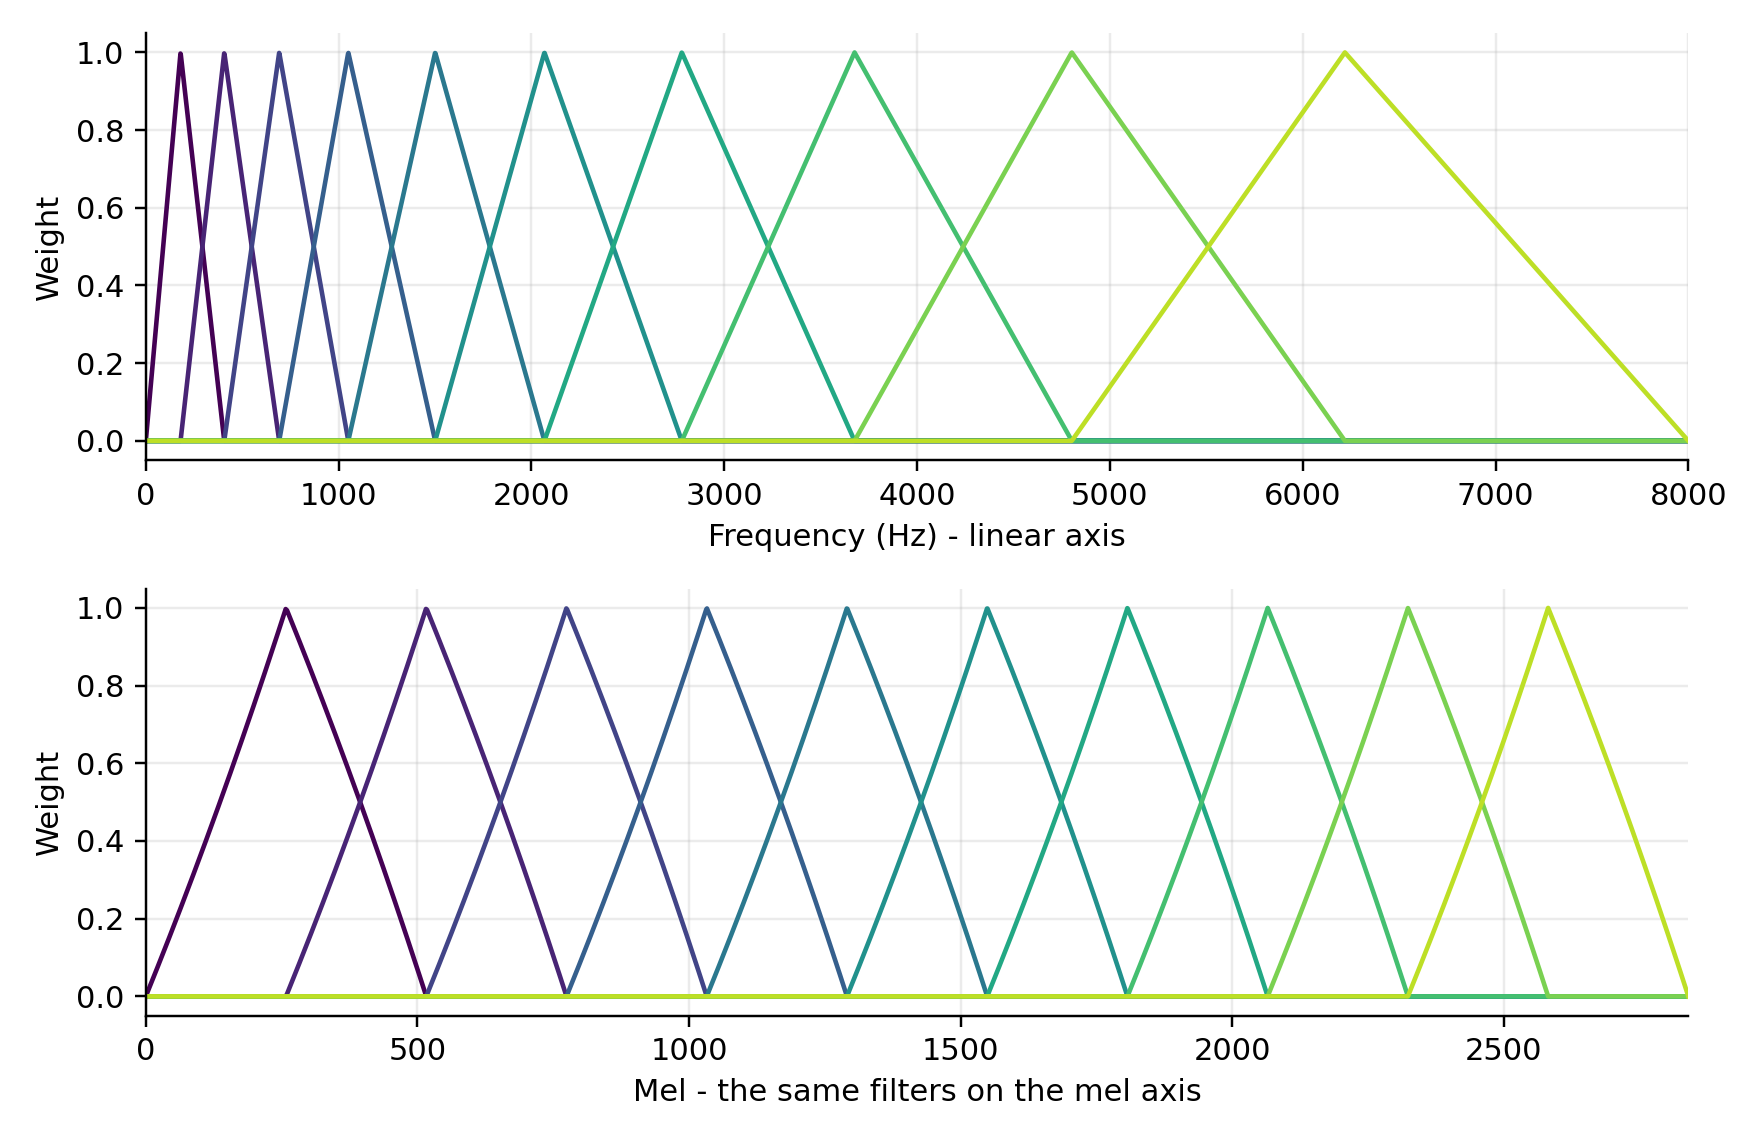
\includegraphics[width=0.9\textwidth]{../assets/figures/ch05-mel-filterbank.png}
  \caption{نمونهٔ یک بانک ده‌فیلتری برای بازهٔ ۰ تا ۸ کیلوهرتز. بالا: روی محور خطی هرتز فیلترها به‌تدریج پهن می‌شوند. پایین: همان فیلترها روی محور مل، مثلث‌هایی یکسان و هم‌فاصله‌اند. (شکل افزوده)}
  \label{fig:fbplot}
\end{figure}

\subsection{تعداد فیلترها}
در کلاس: حدود ۴۰ فیلتر مل رایج است و خروجی هر فریم یک بردار ۴۰‌تایی $\mathbf{M}=[M_1,\ldots,M_{40}]$ است. استاد تأکید کرد ۴۰ مقدار تجربی و متداول است، نه ثابت اجباری. 

\begin{correctionbox}{طیف توان یا اندازه؟}
در کلاس گفته شد اندازهٔ خروجی فوریه در مثلث‌ها ضرب می‌شود. هر دو دیده می‌شوند، اما در تعریف استاندارد \eng{MFCC} فیلترها روی \emph{طیف توان} (مربع اندازه، «انرژی هر باند») اعمال می‌شوند.
\end{correctionbox}

\begin{exambox}{پرسش و پاسخ: آیا با ادغام فرکانس‌ها اطلاعات از دست نمی‌رود؟}
چرا، عمداً اطلاعات را \emph{خلاصه} می‌کنیم. هدف نگه‌داشتن طیف اصلی نیست، ساختن نمایشی مناسب‌تر برای گفتار است: تفکیک ریز فرکانس‌های بالا از دید ادراک اهمیت کمتری دارد و هم‌پوشانی از حذف ناگهانی اطلاعات مرزی جلوگیری می‌کند.
\end{exambox}

%====================================================================
\section{ادراک غیرخطی بلندی صدا و لگاریتم}
%====================================================================

گوش در \emph{شدت} هم غیرخطی است: اگر شدت فیزیکی ۱۰۰ برابر شود، صدا را ۱۰۰ برابر بلندتر حس نمی‌کنیم، بلکه فقط چند برابر. این ویژگی به گوش اجازه می‌دهد با گسترهٔ بسیار وسیعی از شدت‌ها کار کند.

برای وارد کردن این ویژگی از خروجی هر فیلتر مل لگاریتم می‌گیریم:
\[
L_i=\log(M_i),\qquad \mathbf{L}=[\log M_1,\ldots,\log M_{40}].
\]
لگاریتم تغییرات بزرگ را فشرده می‌کند: $\log_{10}(10)=1$، $\log_{10}(100)=2$، $\log_{10}(1000)=3$؛ ورودی ۱۰۰ برابر شده ولی خروجی فقط از ۱ به ۳ رسیده است. در کلاس تأکید شد در این مرحله فقط روی \emph{شدت} لگاریتم می‌گیریم و به زیر و بمی کاری نداریم.

\begin{correctionbox}{لگاریتم، تقریبی از بلندی؛ نه خود بلندی}
لگاریتم مدلی ساده برای فشردگی بلندی است، نه رابطهٔ دقیق آن. قانون توانی استیونز می‌گوید بلندی تقریباً با $I^{0.3}$ متناسب است: ۱۰۰ برابر شدن شدت، بلندی را حدود $100^{0.3}\approx4$ برابر می‌کند.
\end{correctionbox}

\begin{warningbox}{لگاریتم صفر!}
اگر خروجی فیلتر صفر باشد (مثلاً سکوت دیجیتال)، $\log 0=-\infty$ می‌شود. در عمل مقدار کوچک $\varepsilon$ اضافه می‌شود: $L_i=\log(M_i+\varepsilon)$.
\end{warningbox}

\begin{table}[htbp]
\centering
\caption{دو ادراک غیرخطی شنوایی و راه‌حل‌های متناظر در \eng{MFCC}.}
\begin{tabular}{p{5.5cm}p{6cm}}
\toprule
\textbf{مسئله} & \textbf{راه‌حل} \\
\midrule
ادراک غیرخطی تفاوت فرکانس‌ها & مقیاس مل و بانک فیلتر مل \\
ادراک غیرخطی تغییرات شدت صوت & تبدیل لگاریتمی \\
\bottomrule
\end{tabular}
\end{table}

%====================================================================
\section{افزونگی ویژگی‌ها و تبدیل کسینوسی گسسته}
%====================================================================

اکنون برای هر فریم ۴۰ عدد داریم، اما چون فیلترهای مجاور هم‌پوشان‌اند، این اعداد \emph{هم‌بستگی} (\eng{Correlation}) زیادی دارند و بخشی از اطلاعاتشان تکراری است. می‌خواهیم تعداد ویژگی‌ها را کم کنیم و بخش مهم اطلاعات را نگه داریم.

استاد این مرحله را شهودی «یک تبدیل فوریهٔ دیگر» روی همین ۴۰ عدد توصیف کرد: عملاً \term{تبدیل کسینوسی گسسته}{Discrete Cosine Transform, DCT}. از خروجی آن ۱۲ یا ۱۳ ضریب اول نگه داشته می‌شود و همین‌ها \eng{MFCC} نام دارند. برای $M$ مقدار لگاریتمی:
\[
c_n=\sum_{m=1}^{M} L_m\cos\!\Big(\frac{\pi n\,(m-\tfrac12)}{M}\Big),\qquad n=0,1,\ldots,12 .
\]
دنبالهٔ $L_m$ مانند «سیگنالی» است که متغیر مستقل آن به‌جای زمان، شمارهٔ فیلتر (فرکانس) است. ضرایب پایین ($n$ کوچک) شکل کلی طیف (پوش) را و ضرایب بالا تغییرات سریع و ریز را توصیف می‌کنند.

\begin{correctionbox}{چرا DCT هم‌بستگی را کم می‌کند؟}
پایه‌های \eng{DCT} متعامدند و برای دنباله‌های هموار و به‌شدت هم‌بسته تقریب بسیار خوبی از تبدیل کارونن‌لوو (\eng{PCA}) هستند: بیشتر انرژی در چند ضریب نخست جمع می‌شود و ضرایب تقریباً ناهم‌بسته‌اند. تفاوت با \eng{PCA}: پایه‌های \eng{DCT} ثابت‌اند و از داده آموخته نمی‌شوند.
\end{correctionbox}

\begin{addedbox}{مثال عددی: فشردگی انرژی با DCT}
دنبالهٔ هموار $\mathbf{x}=[5,\,5.2,\,4.9,\,8,\,8.1,\,7.9]$ (شبیه دنبالهٔ تخته) دو سطح تقریباً ثابت دارد. \eng{DCT-II} متعامد آن $\mathbf{c}\approx[15.96,\,-3.26,\,0.00,\,1.27,\,-0.23,\,-0.98]$ است؛ دو ضریب اول حدود \textbf{۹۹٪} انرژی را دارند و بازسازی از همین دو ضریب شکل کلی (پایین در ابتدا، بالا در انتها) را حفظ می‌کند. این منطق نگه‌داشتن ۱۲ تا ۱۳ ضریب از ۴۰ مقدار است.
\end{addedbox}

\subsection{چرا ۱۲ یا ۱۳ ضریب؟}
انتخاب تجربی است. تعداد فیلترها (حدود ۴۰) و تعداد ضرایب (۱۲ یا ۱۳؛ گاهی ۵ یا بیشتر) هر دو \term{ابرپارامتر}{Hyperparameter}اند و بر اساس عملکرد سیستم تنظیم می‌شوند. کاهش از ۴۰ مقدار به ۱۳ ضریب یعنی حدود $32.5$٪ ابعاد اولیه.

\begin{exambox}{پرسش و پاسخ: آیا انتخاب ۱۲ یا ۱۳ ضریب اثبات ریاضی دارد؟}
خیر؛ تجربی است و یک ابرپارامتر قابل‌تنظیم است.
\end{exambox}

%====================================================================
\section{کپستروم و روایت تاریخی تحلیل کپسترال}
%====================================================================

واژهٔ \term{کپستروم}{Cepstrum} از جابه‌جایی چهار حرف نخست \eng{Spectrum} ساخته شده است؛ مفهوم آن در کلاس «طیفِ یک طیف» بود. محور مستقل آن \term{کوفرنسی}{Quefrency} نام دارد و واحدش از جنس زمان است.

\textbf{روایت تاریخی کلاس:} در جنگ سرد، آمریکا می‌خواست از روی امواج ثبت‌شده تشخیص دهد رویداد زلزله بوده یا آزمایش هسته‌ای شوروی. اعمال تبدیل دوم روی اطلاعات طیفی الگوهایی را آشکار می‌کرد که در طیف اولیه به‌آسانی دیده نمی‌شد. نکتهٔ اصلی: گاهی با تبدیل دوبارهٔ یک نمایش طیفی، اطلاعاتی آشکار می‌شود که در نمایش اولیه پنهان است.

\begin{correctionbox}{دقت تاریخی}
اصل روایت درست است: کپستروم را \eng{Bogert}، \eng{Healy} و \eng{Tukey} در ۱۹۶۳ برای تشخیص \emph{پژواک} در رکوردهای لرزه‌نگاری معرفی کردند و انگیزهٔ آن با تفکیک زلزله از انفجار مرتبط دانسته می‌شود. اما \eng{MFCC} را بعدها (۱۹۸۰) \eng{Davis} و \eng{Mermelstein} برای تشخیص گفتار معرفی کردند و ربط مستقیمی با لرزه‌شناسی ندارد. (واژه‌های \eng{quefrency}، \eng{lifter} و \eng{liftering} هنوز به کار می‌روند.)
\end{correctionbox}

\textbf{شهود کپستروم:} کپستروم حقیقی $c[n]=\mathrm{IDFT}\{\log|\mathrm{DFT}\{x[n]\}|\}$ است. در گفتار واک‌دار، هارمونیک‌های $F_0$ در لگاریتم طیف موج‌هایی ریز می‌سازند که در کپستروم به قله‌ای در کوفرنسی $1/F_0$ تبدیل می‌شوند، در حالی که پوش طیف (مجرای صوتی و فرمنت‌ها) در کوفرنسی‌های پایین می‌ماند؛ بدین‌ترتیب منبع و فیلتر از هم جدا می‌شوند.

\begin{correctionbox}{کپستروم کلاسیک و DCT در MFCC یکسان نیستند}
\eng{DCT} در \eng{MFCC} نسخه‌ای از همان ایده است، نه دقیقاً همان عمل: در کپستروم کلاسیک از لگاریتم \emph{طیف کامل} با \eng{IDFT} تبدیل می‌گیریم، ولی در \eng{MFCC} ابتدا طیف با بانک فیلتر مل فشرده می‌شود، سپس لگاریتم و \eng{DCT}. با نگه‌داشتن فقط ضرایب اول، پوش طیف (شکل مجرا، یعنی واج) حفظ می‌شود و \eng{MFCC} کمتر به $F_0$ حساس است.
\end{correctionbox}

%====================================================================
\section{مسیر کامل استخراج MFCC}
%====================================================================

مسیر مفهومی کلاس: سیگنال گفتار $\leftarrow$ تبدیل فوریه $\leftarrow$ بانک فیلتر مل $\leftarrow$ لگاریتم $\leftarrow$ \eng{DCT} $\leftarrow$ انتخاب ضرایب اول. در پیاده‌سازی واقعی چند مرحلهٔ دیگر (که فریم‌بندی و پنجره‌گذاری‌شان را از بحث اسپکتروگرام می‌شناسیم) هم افزوده می‌شود:

\begin{figure}[htbp]
  \centering
  \begin{tikzpicture}[rtl, node distance=0.5cm, blk/.style={draw, rounded corners, minimum width=4.3cm, minimum height=0.75cm, align=center, fill=blue!7, font=\small}, note/.style={font=\footnotesize, text width=5.8cm, align=right}]
    \node[blk, fill=gray!15] (n0) {\RL{سیگنال گفتار (\lr{Waveform})}};
    \node[blk, below=of n0] (n1) {\lr{Pre-emphasis}};
    \node[blk, below=of n1] (n2) {\lr{Framing (25 ms / hop 10 ms)}};
    \node[blk, below=of n2] (n3) {\lr{Windowing (Hamming)}};
    \node[blk, below=of n3] (n4) {\lr{FFT} $\rightarrow$ \lr{Power spectrum}};
    \node[blk, below=of n4, fill=orange!15] (n5) {\lr{Mel Filterbank (40 filters)}};
    \node[blk, below=of n5, fill=orange!15] (n6) {\lr{Log}};
    \node[blk, below=of n6, fill=orange!15] (n7) {\lr{DCT}};
    \node[blk, below=of n7, fill=green!12] (n8) {\lr{MFCC} $c_1\ldots c_{12}$ + \lr{energy}};
    \node[blk, below=of n8, fill=green!12] (n9) {\lr{$\Delta$, $\Delta\Delta$ $\Rightarrow$ 39 features/frame}};
    \foreach \a/\b in {0/1,1/2,2/3,3/4,4/5,5/6,6/7,7/8,8/9} \draw[-{Latex}] (n\a) -- (n\b);
    \node[note, left=0.6cm of n1] {\RL{تقویت فرکانس‌های بالا}};
    \node[note, left=0.6cm of n2] {\RL{هر فریم ۴۰۰ نمونه در \lr{16 kHz}}};
    \node[note, left=0.6cm of n3] {\RL{کاهش نشتی طیفی لبه‌های فریم}};
    \node[note, left=0.6cm of n4] {\lr{512-point FFT $\rightarrow$ 257 bins}};
    \node[note, left=0.6cm of n5] {\RL{بخش ادراکی ۱: مقیاس مل}};
    \node[note, left=0.6cm of n6] {\RL{بخش ادراکی ۲: ادراک لگاریتمی بلندی}};
    \node[note, left=0.6cm of n7] {\RL{حذف هم‌بستگی و فشرده‌سازی}};
    \node[note, left=0.6cm of n9] {\RL{ویژگی‌های پویا (سرعت و شتاب)}};
  \end{tikzpicture}
  \caption{نمودار بلوکی استخراج \eng{MFCC} تا بردار ویژگی هر فریم. بلوک‌های نارنجی بخش‌هایی‌اند که در این جلسه تدریس شد. (شکل افزوده)}
  \label{fig:mfccpipe}
\end{figure}

\begin{correctionbox}{مراحل پیش‌پردازش در کلاس}
فهرست کلاس فقط هستهٔ ادراکی را نشان می‌دهد؛ پیش‌تأکید (فیلتر بالاگذر $y[n]=x[n]-\alpha x[n-1]$ با $\alpha\approx0.97$)، فریم‌بندی (۲۵ میلی‌ثانیه با گام ۱۰ میلی‌ثانیه)، پنجره‌گذاری همینگ و ضرایب دلتا و دلتا-دلتا (تغییرات زمانی؛ ۱۳+۱۳+۱۳ = بردار ۳۹ بعدی) نیز به‌طور استاندارد جزو زنجیره‌اند. «\eng{MFCC} ۱۲تایی» یعنی $c_1$ تا $c_{12}$ و «۱۳تایی» یعنی افزودن $c_0$ (یا انرژی)؛ این علت دوگانهٔ «۱۲ یا ۱۳» در سخنان استاد است.
\end{correctionbox}

\begin{figure}[htbp]
  \centering
  \fbox{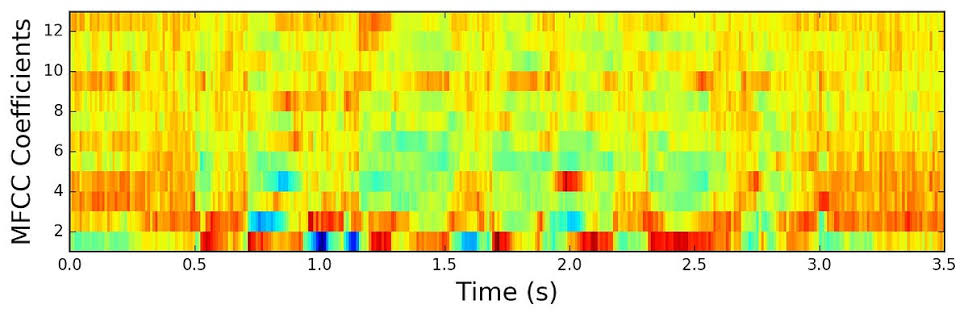
\includegraphics[width=0.85\textwidth]{../assets/figures/ch05-mfcc-matrix.png}}
  \caption{نمایش ماتریسی \eng{MFCC}: محور افقی زمان، محور عمودی شمارهٔ ضریب (۱ تا ۱۳) و رنگ مقدار هر ضریب در هر فریم است. \textit{(برگرفته از تختهٔ کلاس)}}
  \label{fig:mfccmat}
\end{figure}

\begin{exambox}{جمع‌بندی سه مسئله و راه‌حل در تخته}
\begin{enumerate}
  \item \textbf{بانک فیلتر مل}: ادراک غیرخطی فرکانس $\Leftarrow$ مقیاس مل.
  \item \textbf{لگاریتم}: ادراک غیرخطی بلندی (۱۰۰ برابر بلندتر را فقط چند برابر بلندتر حس می‌کنیم) $\Leftarrow$ لگاریتم انرژی مل.
  \item \textbf{\eng{DCT}}: ۴۰ عدد شبیه و تکراری $\Leftarrow$ \eng{DCT} و برداشتن ۱۲ تا ۱۳ ضریب اول.
\end{enumerate}
\end{exambox}

%====================================================================
\section{کاربردهای MFCC}
%====================================================================

ماتریس \eng{MFCC} (برای هر فریم یک بردار ضریب) جایگزین نمایش‌های حجیم‌تر سیگنال می‌شود. کاربردهای مطرح‌شده در کلاس:
\begin{itemize}
  \item \textbf{مقایسهٔ سیگنال‌ها}: استخراج \eng{MFCC} دو سیگنال و سنجش شباهت (مثلاً با هم‌بستگی).
  \item \textbf{تحلیل صدای سرفه}: مقایسهٔ سرفهٔ افراد مبتلا به یک بیماری تنفسی (مانند کووید-۱۹) با سایرین و آموزش یک طبقه‌بند؛ نشان می‌دهد \eng{MFCC} فقط برای تشخیص کلمات نیست.
  \item \textbf{تبدیل گفتار به متن}: به‌جای موج خام، ویژگی‌های آکوستیکی مانند \eng{MFCC} به مدل داده می‌شود؛ ویژگی‌های دیگر (مثل \eng{pitch}) در صورت نیاز جداگانه استخراج می‌شوند.
\end{itemize}

\begin{warningbox}{هشدار}
استخراج \eng{MFCC} یا مشاهدهٔ یک هم‌بستگی به‌تنهایی برای تشخیص بیماری کافی نیست؛ داده‌های معتبر، آموزش و ارزیابی مدل لازم است. مقایسهٔ مستقیم \eng{MFCC} سیگنال‌هایی با طول یا سرعت متفاوت هم به هم‌ترازسازی زمانی (مثلاً \eng{DTW}) یا خلاصه‌سازی آماری نیاز دارد.
\end{warningbox}

%====================================================================
\section{MFCC در یادگیری ماشین و یادگیری عمیق}
%====================================================================

\begin{itemize}
  \item \textbf{آیا استخراج \eng{MFCC} یادگیری ماشین است؟} استاد تأکید کرد خیر: مجموعه‌ای از عملیات ثابت پردازش سیگنال (طیف، بانک فیلتر، لگاریتم، \eng{DCT}، انتخاب ضرایب) با پارامترهای مشخص است و به آموزش روی داده نیاز ندارد؛ اما خروجی‌اش را می‌توان به یک مدل یادگیری ماشین داد.
  \item \textbf{مقایسه با \eng{PCA}} (پرسش دانشجو): از نظر هدف (نمایش فشرده) شبیه‌اند، اما \eng{MFCC} زنجیرهٔ ثابت تبدیل‌هاست و \eng{PCA} روشی آماری است که مؤلفه‌ها را از داده می‌آموزد. اگر پس از لگاریتم مل از \eng{PCA} استفاده شود، دیگر با تعریف متداول \eng{MFCC} کار نمی‌کنیم.
  \item \textbf{در یادگیری عمیق}: می‌توان \eng{MFCC} را هم به مدل داد، چون نمایشی ساختاریافته و فشرده است؛ انتخاب میان موج خام، طیف و \eng{MFCC} به مسئله و عملکرد تجربی بستگی دارد.
\end{itemize}

\begin{correctionbox}{روند امروز: \eng{log-mel} به‌جای \eng{MFCC}}
مدل‌های عصبی امروزی (مانند \eng{Whisper}) بیشتر از لگاریتم انرژی‌های مل (\eng{log-mel}) استفاده می‌کنند و \eng{DCT} را حذف می‌کنند، چون شبکه خودش هم‌بستگی‌ها را می‌آموزد و \eng{DCT} ترتیب فرکانسی را به هم می‌زند. برخی مدل‌ها (مانند \eng{wav2vec 2.0}) از موج خام شروع می‌کنند. \eng{MFCC} همچنان در مدل‌های کلاسیک (\eng{GMM-HMM})، مدل‌های سبک و داده‌های کم کاربرد دارد.
\end{correctionbox}

%====================================================================
\section{جمع‌بندی}
%====================================================================

گوش هم فرکانس را غیرخطی درک می‌کند (نقشهٔ تونوتوپیک، تفکیک بیشتر در بم) و هم شدت را. برای اولی از مقیاس مل و بانک فیلتر مثلثی هم‌پوشان با عرض‌های رشدیابنده و برای دومی از لگاریتم استفاده کردیم. چون ۴۰ انرژی لگاریتمی مل بسیار هم‌بسته‌اند، با \eng{DCT} به ضرایب کپسترال تبدیل شدند و ۱۲ تا ۱۳ ضریب اول نگه داشته شد:
\[
\text{\lr{Speech Signal}}\to\text{\lr{Spectrum}}\to\text{\lr{Mel Filters}}\to\log\to\text{\lr{DCT}}\to\text{\lr{MFCC}} .
\]
نتیجهٔ اصلی: به‌جای همهٔ اطلاعات طیفی، نمایشی فشرده و مناسب گفتار می‌سازیم که ویژگی‌های ادراکی گوش در طراحی آن لحاظ شده است.

\begin{exambox}{نکات مهم برای مرور و امتحان}
\begin{enumerate}
  \item تفاوت $F_0$ با \eng{Pitch} و تفاوت شدت فیزیکی با بلندی ادراک‌شده را بدانید.
  \item نقشهٔ تونوتوپیک (قاعده $\Leftrightarrow$ فرکانس بالا، رأس $\Leftrightarrow$ فرکانس پایین) و پیامد آن (کم‌شنوایی فرکانس بالا با سن) را بشناسید.
  \item توضیح دهید چرا ادراک فرکانس خطی نیست (۱۰۰ تا ۲۰۰ در برابر ۵۱۰۰ تا ۵۲۰۰ هرتز)؛ فرمول $m=2595\log_{10}(1+f/700)$.
  \item بدانید چرا عرض فیلترهای مل در فرکانس‌های بالا بیشتر می‌شود، و هم‌پوشانی و وزن‌دهی مثلثی را توضیح دهید؛ خروجی یک فیلتر را حساب کنید (مثال $M_1=13$).
  \item دلیل لگاریتم از انرژی فیلترها را توضیح دهید.
  \item نقش \eng{DCT} (کاهش هم‌بستگی و فشرده‌سازی) و دلیل نگه‌داشتن ۱۲ یا ۱۳ ضریب را بدانید؛ تعداد فیلترها (حدود ۴۰) و ضرایب ابرپارامترند، نه اجباری.
  \item مسیر استخراج \eng{MFCC} را از سیگنال تا ضرایب نهایی شرح دهید.
  \item \eng{MFCC} (زنجیرهٔ ثابت پردازش سیگنال) را با \eng{PCA} (یادگیری از داده) مقایسه کنید.
  \item معنای واژهٔ کپستروم (جابه‌جایی حروف \eng{Spectrum}، «طیفِ طیف») را بدانید.
\end{enumerate}
\end{exambox}
